\documentclass{article}

\PassOptionsToPackage{numbers, compress}{natbib}
\usepackage[preprint]{neurips_2026}

\usepackage[utf8]{inputenc}
\usepackage[T1]{fontenc}
\usepackage{hyperref}
\usepackage{url}
\usepackage{booktabs}
\usepackage{amsfonts}
\usepackage{amsmath}
\usepackage{nicefrac}
\usepackage{microtype}
\usepackage{xcolor}
\usepackage{graphicx}
\usepackage{subcaption}
\usepackage{placeins}

\setlength{\textfloatsep}{4pt plus 1pt minus 1pt}
\setlength{\floatsep}{4pt plus 1pt minus 1pt}
\setlength{\intextsep}{4pt plus 1pt minus 1pt}
\setlength{\abovecaptionskip}{2pt}
\setlength{\belowcaptionskip}{0pt}
\setlength{\dbltextfloatsep}{4pt}
\setlength{\bibsep}{6pt plus 0.3ex}

\graphicspath{{../figures/}}

\title{A Hybrid Spatio-Temporal Pipeline for NYC Crash Hotspot Discovery and Severity Prediction}

\author{%
  Vishal Nagamalla\thanks{Equal contribution.} \\
  Department of Computer Science\\
  Rutgers University\\
  \texttt{vn218@scarletmail.rutgers.edu} \\
  \And
  Pranav Arra\footnotemark[1] \\
  Department of Computer Science\\
  Rutgers University\\
  \texttt{psa39@scarletmail.rutgers.edu} \\
  \And
  Logan Sharrott\footnotemark[1] \\
  Department of Computer Science\\
  Rutgers University\\
  \texttt{ls1428@scarletmail.rutgers.edu} \\
}

\begin{document}

\maketitle
\vspace{-1.5em}

\begin{abstract}
The data science workflow outlined in this paper addresses two issues in
existing research and practice. First, road traffic accidents are a
significant hazard in densely populated areas such as cities, but the vast
majority of city governments do not provide open access to their accident
databases; second, although most researchers use supervised learning
techniques to predict crash severity; a few studies have employed or
discussed unsupervised geospatial analysis to identify high-risk areas of
the city. This paper presents a pipeline of data science processes applied
to the New York City Motor Vehicle Collisions Dataset (2021-2022), which
applies both unsupervised geospatial clustering and supervised classification
of crash severity. The process begins with a single preprocessing stage that
prepares the NYC MVC crash records into four feature categories:
temporal/cyclical time encoding; weather coding; spatial coding; and a
daily-weather join. After applying the Elbow and Silhouette diagnostics to
the training set of crash locations to find $k = 4$, the researcher uses
k-means to cluster crash locations into four groups and validates these
results against a DBSCAN baseline based on the Haversine distance. Following
validation, the researcher defines the cluster identity as a categorical
variable and feeds it into three sequential logistic regression, random
forest, and xgboost classifiers to determine whether the crash falls into
the ``serious'' category. Each classifier was trained using methods designed
to correct for the extremely large imbalance of classes found in the
original data (2.75 percent ``serious''). The researcher then evaluated each
model based on performance metrics including Precision-Recall AUC (PR-AUC),
Receiver Operating Characteristic Area Under Curve (ROC-AUC) scores,
Balanced Accuracy, Calibration Statistics, SHAP feature attributions, and a
Feature Group Ablation Test. Overall, there were three key results from this
research: (1)~the four identified K-means clusters cover approximately a
28\% relative difference in serious-crash rates; (2)~Class-Weighted Logistic
Regression produced the highest balanced accuracy (0.585), suggesting that
the choice of how to treat imbalanced classes is significantly more
important than the capacity of the model being used; and (3)~once raw
latitude and longitude are available, gradient-boosted tree models can
already extract the underlying spatial structure on their own, making the
K-means cluster identity largely redundant for them as a feature.
\end{abstract}

\section{Introduction}
\label{sec:intro}

Traffic accidents are among the highest frequency, most impactful public
health events in cities. In addition to publishing hundreds of thousands of
collision reports annually through NYC Open Data~\cite{nyc_collisions}, the
NYC Open Data platform provides collision information about incidents,
which is detailed in both time and space. However, the data itself, while
extensive in detail for location and time, is provided typically in a
non-relational format (i.e., flat CSV file) without being combined with
additional relevant signals such as weather or road geometry; without a
structured management system for the data; and without defined baselines
to connect unsupervised discovery of hotspots to supervised predictions of
accident severity. Consequently, downstream analysis tends to be ``ad hoc,''
difficult to reproduce; and rarely includes suitable metrics that account
for the extreme class imbalance inherent in predicting severe accidents.

This paper outlines an integrated data science workflow from raw feeds of
NYC collision data and weather conditions to a reproducing analytical
object well-suited to answering two complementary queries:
\textit{\textbf{Q1)} Where and at what times do severe accidents occur?}
and
\textit{\textbf{Q2)} Can we use the available contextual attributes to
determine if a particular incident will likely be classified as a severe
accident?}

Our contributions are as follows:
\begin{itemize}
\item Our code and data are entirely reproducible via an easily reproduced
parquet database (SQLite cache), deterministic seed values, as well as a
one-line command to reproduce all figures, tables, and metrics presented
within this
paper.\footnote{Code: \url{https://github.com/Vishal-Nagamalla/Traffic-Hotspot-Final}}
\item Using KMeans clustering (we used Elbow \& Silhouette diagnostic
techniques to find our number of clusters), we performed unsupervised
spatial hotspot detection on the joined crash--weather dataset and measured
how the cluster identities corresponded with rates of serious crashes.
\item We designed a supervised multi-layer classification model
(majority-class baseline; logistic regression; random forest; xgboost;
xgboost + SMOTE; xgboost w/ threshold optimization) based upon a
chronological train-test split and evaluated its performance using PR-AUC,
ROC-AUC, Balanced Accuracy, Calibration Metrics, and SHAP Feature
Attribution analysis.
\item Finally, we conducted an Ablation study to identify the incremental
contribution of each of the four feature groups. The results show that
time-based features are most valuable and that spatial features have very
little additional benefit beyond what can be obtained by knowing
$(\mathrm{lat}, \mathrm{lon})$.
\end{itemize}

\section{Related Work}
\label{sec:related}

We group prior work into three categories that map directly onto the components
of our pipeline: (i)~spatio-temporal clustering of crashes, (ii)~supervised
crash-severity prediction, and (iii)~hybrid frameworks combining clustering and
classification with explainability.

\paragraph{Crash Hotspot Detection.}
Hotspot detection was one of the first use cases for spatial analysis in
road safety. Anderson used K-means clustering along with Kernel Density
Estimation to find high-risk locations based on accidents in
London~\cite{anderson2009kernel}. Prasannakumar extended their work into
GIS-based spatiotemporal approach~\cite{prasannakumar2011spatio}. Recently,
density-based approaches like DBSCAN~\cite{ester1996dbscan} were utilized to
determine local hotspot areas by considering the geometry of the data at
hand. The authors found it beneficial to link crashes to environmental
features (such as weather and POIs), which has already shown promise from
previous studies (Moosavi~\cite{moosavi2019accident}, etc.). This study
follows the same line of research; however, we propose combining both
KMeans and Haversine distance DBSCAN in an integrated pipeline.

\paragraph{Crash Severity Prediction.}
The supervised severity classification has been approached by an assortment
of different models. Abdelwahab et al. (2001) utilize artificial neural
networks to estimate the injury severity for
drivers~\cite{abdelwahab2001modeling}. Iranitalab et al. (2017), conducted a
systematic comparison of a variety of models that include Multinomial Logit
Model, Nearest Neighbor Model, Support Vector Machine, Random Forest Models
using U.S. crash data~\cite{iranitalab2017comparison}. Theofilatos et al.
(2014), reviewed how weather and traffic condition affect injury
severity~\cite{theofilatos2014review}. There are two common themes
throughout the studies on the injury severity classification; first it is
difficult to recover the severity signals from the limited number of
features available post-crash as well as, secondly due to the large class
imbalance that exist within most crash datasets.

\paragraph{Hybrid and Explainable Frameworks.}
A number of studies have begun to combine unsupervised segmentation with
supervised prediction and apply tools for explaining the predictions (such
as SHAP~\cite{lundberg2017shap}), which was originally introduced as a
general framework for interpreting machine-learning models and has since
been used in many other areas including safety analytics. Techniques that
are aware of imbalance (such as SMOTE~\cite{chawla2002smote}) and threshold
tuning, when the positive class is rare, have become standard when working
with imbalanced datasets~\cite{he2009imbalanced}. Our research combines
these concepts by using an unsupervised clustering method to extract spatial
patterns from the data, then applying a tree ensemble classifier
ladder~\cite{breiman2001random, chen2016xgboost} to predict crash severity
using both the original features and the cluster identity that was produced
by the clustering step, and finally using SHAP to provide explanations for
the top performing tree-based model.

\section{Methodology}
\label{sec:method}

\subsection{Datasets}
We used two publicly available datasets. The NYC Motor Vehicle Collisions
dataset~\cite{nyc_collisions}, was converted into a CSV file with each row
representing one motor vehicle collision, which included the date/time of
the crash, Borough, Zip code, Latitude/Longitude of the location where the
crash occurred, On/Off street name(s), Number of persons Injured or Killed.
The NYC Hourly Weather~\cite{nyc_weather} dataset includes data on hourly
temperature, Precipitation, Rain, Cloud Cover and Wind Speed. However
although the Crash Data spans from 2021-2025 and the weather data spans
from 2016-2022, we utilized both datasets for the years 2021-2022 (a two
year span) so that there would be a weather context associated with each
crash. After filtering out bad time stamps, coordinates that were outside
the bounds of the NYC geographic area, and after successfully joining the
weather data with the crash data, we retained \textbf{177,313 crashes} and
\textbf{2,490 weather days} of data. Of those crashes approximately 42k
had an unknown value for the borough field; they will be modeled but will
not be included when providing the results by borough shown in
Table~\ref{tab:borough}.

\subsection{Data Preprocessing}
\label{sec:preproc}
We apply the same pipeline for cleaning data as we do to preprocess our
training data. The entire pipeline is encapsulated in a single sklearn
\texttt{ColumnTransformer}/\texttt{Pipeline} so that no transform will ever
see more than the one training fold and therefore cannot leak any test
information.

\paragraph{Cleaning.} We exclude crash records whose timestamp could not be
parsed, which have missing coordinates, or coordinates that are outside of
New York City's bounding box $(-74.3, -73.6) \times (40.4, 41.0)$, and then
remove duplicates based on the unique collision id.
\paragraph{Severity Label.} We define a binary label
$y_i = \mathbf{1}\{\text{deaths}_i > 0 \;\lor\; \text{injuries}_i \geq 3\}$,
matching the operational definition of a serious crash used by NYC's Vision
Zero program. The serious rate on the joined dataset is $0.0275$.
\paragraph{Weather Aggregation.} Because the source weather feed is hourly,
we aggregate to a daily record with maximum, minimum, and mean temperature
(in $^\circ$F), summed precipitation (in mm), summed rain, mean cloud cover,
and maximum wind speed. We also derive boolean buckets:
$\texttt{is\_rainy}$ (precip $>$ 1\,mm), $\texttt{is\_heavy\_rain}$
(precip $>$ 10\,mm), $\texttt{is\_freezing}$ ($T_{\min} \leq 32^\circ$F),
$\texttt{is\_hot}$ ($T_{\max} \geq 85^\circ$F), $\texttt{is\_cloudy}$, and
$\texttt{is\_windy}$.
\paragraph{Encoding cyclical time attributes.} The date and time of every
incident was analyzed by breaking it down into three main parts. Hour, Day
of Week, Month were calculated for all incidents. Each part of this
information was represented using two separate numbers that corresponded to
their sine and cosine values respectively at different frequencies such
that, the same frequency is used for 12 o'clock AM and 11 o'clock PM. In
addition to the previously mentioned number encoding, an integer
representation of hour was kept in order to be able to create histograms.
Flags representing if a collision occurred during a weekend, during rush
hours or during nighttime where added to the data as well.
\paragraph{Adding Spatial Information.} A spatial distance attribute called
\texttt{dist\_to\_midtown\_km} was created using the Euclidean distance
formula to calculate distances from a given point. This distance measure
represents how far away in kilometers an incident location is from Times
Square. The coordinates for Times Square are (40.7580, -73.9855). Two
additional attributes \texttt{lat\_bin} and \texttt{lon\_bin} hold a
$0.01^\circ$ grid identifier for latitude and longitude as a coarse spatial
grouping signal.
\paragraph{Using One-Hot and Standardization Transforms.} All boroughs have
been one-hot encoded. Also in our second model (cluster-augmented), all
cluster ids obtained via k-means will be one-hot encoded. As for
standardizing the numerical data, median imputation will be applied to
replace missing values, then the means of the numerical variables will be
subtracted and divided by the standard deviations in order to obtain the
desired distribution. These transformations will be fitted to the training
set of the split over time.
\paragraph{Train/Test Split.} In order to follow established guidelines
within the field of spatiotemporal prediction, the data was split based on
time. We used the first 80\% of all crashes ordered by
\texttt{crash\_datetime} as our training set. The last 20\% of all crashes
were placed into our test set. The majority of the training set that is
90\% was then used to fit the model. A remaining 10\% of the training set
was held out as an internal validation slice to allow us to find optimal
thresholds.

\subsection{Hotspot Discovery via KMeans and DBSCAN}
\label{sec:cluster}
We apply unsupervised clustering in $(\text{latitude}, \text{longitude})$
space, fitted on the training fold only.

\paragraph{Choosing $k$ for KMeans.} We sweep $k\in\{2,\dots,12\}$ and report
both the within-cluster sum-of-squares (Elbow) and silhouette score
(Figure~\ref{fig:diagnostics}). The silhouette is maximized at $k\!=\!4$
($s\!=\!0.465$), which we adopt for the rest of the paper.

\paragraph{KMeans Objective.} KMeans~\cite{macqueen1967kmeans} minimizes
\begin{equation}
\mathcal{L}_{\text{KMeans}}(\{\mu_j\}) =
\sum_{j=1}^{k}\sum_{x\in C_j}\|x - \mu_j\|_2^2 ,
\label{eq:kmeans}
\end{equation}
where $\{\mu_j\}$ are cluster centroids and $\{C_j\}$ are the cluster
assignments. The cluster identity assigned to each crash, $c_i \in \{0,
\dots, 3\}$, is then exposed to the downstream classifier as a one-hot
feature.

\paragraph{DBSCAN Comparison.} As a non-parametric, density-based
baseline~\cite{ester1996dbscan}, we run DBSCAN on a 25,000-crash sample of the
training fold using the Haversine metric with $\varepsilon = 0.5$\,km and
$\texttt{min\_samples} = 50$. DBSCAN identifies 31 clusters and labels
8,664 (35\%) of the sample as noise, indicating that the underlying density
field is highly heterogeneous and that a coarser KMeans-style partitioning is
better suited to use as a categorical feature.

\subsection{Severity Prediction Models}
\label{sec:models}
We approach severity prediction as binary classification and train a five-step
ladder, all under the chronological split.

\paragraph{Majority Baseline.} Always predict 0. This gives high accuracy
($\approx 0.97$) and zero recall on the serious class -- a useful reference
for how misleading raw accuracy can be under imbalance.

\paragraph{Logistic Regression.} A class-weighted logistic regression
\begin{equation}
P(y=1 \mid x) = \sigma(\beta_0 + \beta^{\top} x),
\quad \mathcal{L} = -\sum_i w_{y_i}\bigl[y_i\log p_i + (1-y_i)\log(1-p_i)\bigr],
\label{eq:logreg}
\end{equation}
with $w_1 / w_0 = N_0 / N_1$ to handle imbalance.

\paragraph{Random Forest.} A bagged ensemble of decision
trees~\cite{breiman2001random} with $n_{\text{est}}\!=\!300$,
$\texttt{max\_depth}\!=\!20$, and $\texttt{class\_weight}\!=\!$
\texttt{balanced\_subsample}.

\paragraph{XGBoost.} Gradient-boosted trees~\cite{chen2016xgboost} with
$n_{\text{est}}\!=\!400$, $\texttt{max\_depth}\!=\!6$,
$\texttt{learning\_rate}\!=\!0.1$, and a positive-class weight
$\texttt{scale\_pos\_weight} = N_0/N_1 \approx 36$. The optimisation objective
is
\begin{equation}
\mathcal{L}_{\text{XGB}} = \sum_i \ell\bigl(y_i, \hat{f}(x_i)\bigr) + \sum_{m=1}^{M} \Omega(h_m),
\label{eq:xgb}
\end{equation}
where $\ell$ is binary log-loss and $\Omega$ regularizes tree complexity.

\paragraph{XGBoost + SMOTE.} We fit the same XGBoost on training features
re-sampled with the Synthetic Minority Over-sampling
Technique~\cite{chawla2002smote}.

\paragraph{XGBoost + Threshold Tuning.} Holding the trained XGBoost fixed, we
search the decision threshold $\tau$ that maximizes the F1 score of the
serious class on the held-out validation slice, and evaluate at that threshold
on the test set.

\paragraph{Feature-Group Ablation.} For Logistic Regression, Random Forest, and
XGBoost we run four feature sets:
\textsc{time-only}, \textsc{+weather}, \textsc{+weather+spatial},
and \textsc{+weather+spatial+cluster (full)}. This isolates the marginal
contribution of weather, the radial spatial feature, and the KMeans cluster
identity.

\section{Experiments \& Results}
\label{sec:results}

\subsection{Evaluation Metrics}
We evaluate using accuracy, balanced accuracy, precision/recall/F1 for the
serious class, ROC-AUC, and PR-AUC. Because the serious class accounts for only
2.75\% of crashes, accuracy and ROC-AUC are insufficient on their own and we
emphasize PR-AUC, balanced accuracy, and per-class recall.

\subsection{Hotspot Discovery}
Figure~\ref{fig:diagnostics} reports the KMeans Elbow and Silhouette
diagnostics: silhouette peaks at $k\!=\!4$ ($s = 0.465$). The resulting cluster
map (Figure~\ref{fig:cluster_map}) recovers a recognizable Manhattan-South
Bronx cluster (centroid 40.82, $-$73.90), a Brooklyn-South cluster (40.68,
$-$73.95), an Eastern Queens cluster (40.70, $-$73.80), and a Staten Island
cluster (40.60, $-$74.13). The serious-crash rate varies from 2.50\% in the
Brooklyn-South cluster to 3.21\% in the Eastern Queens cluster -- an
approximately 28\% relative gap that justifies the cluster id as a candidate feature
(Figure~\ref{fig:cluster_severity}).

\begin{figure}[h]
\begin{subfigure}{0.66\linewidth}\centering
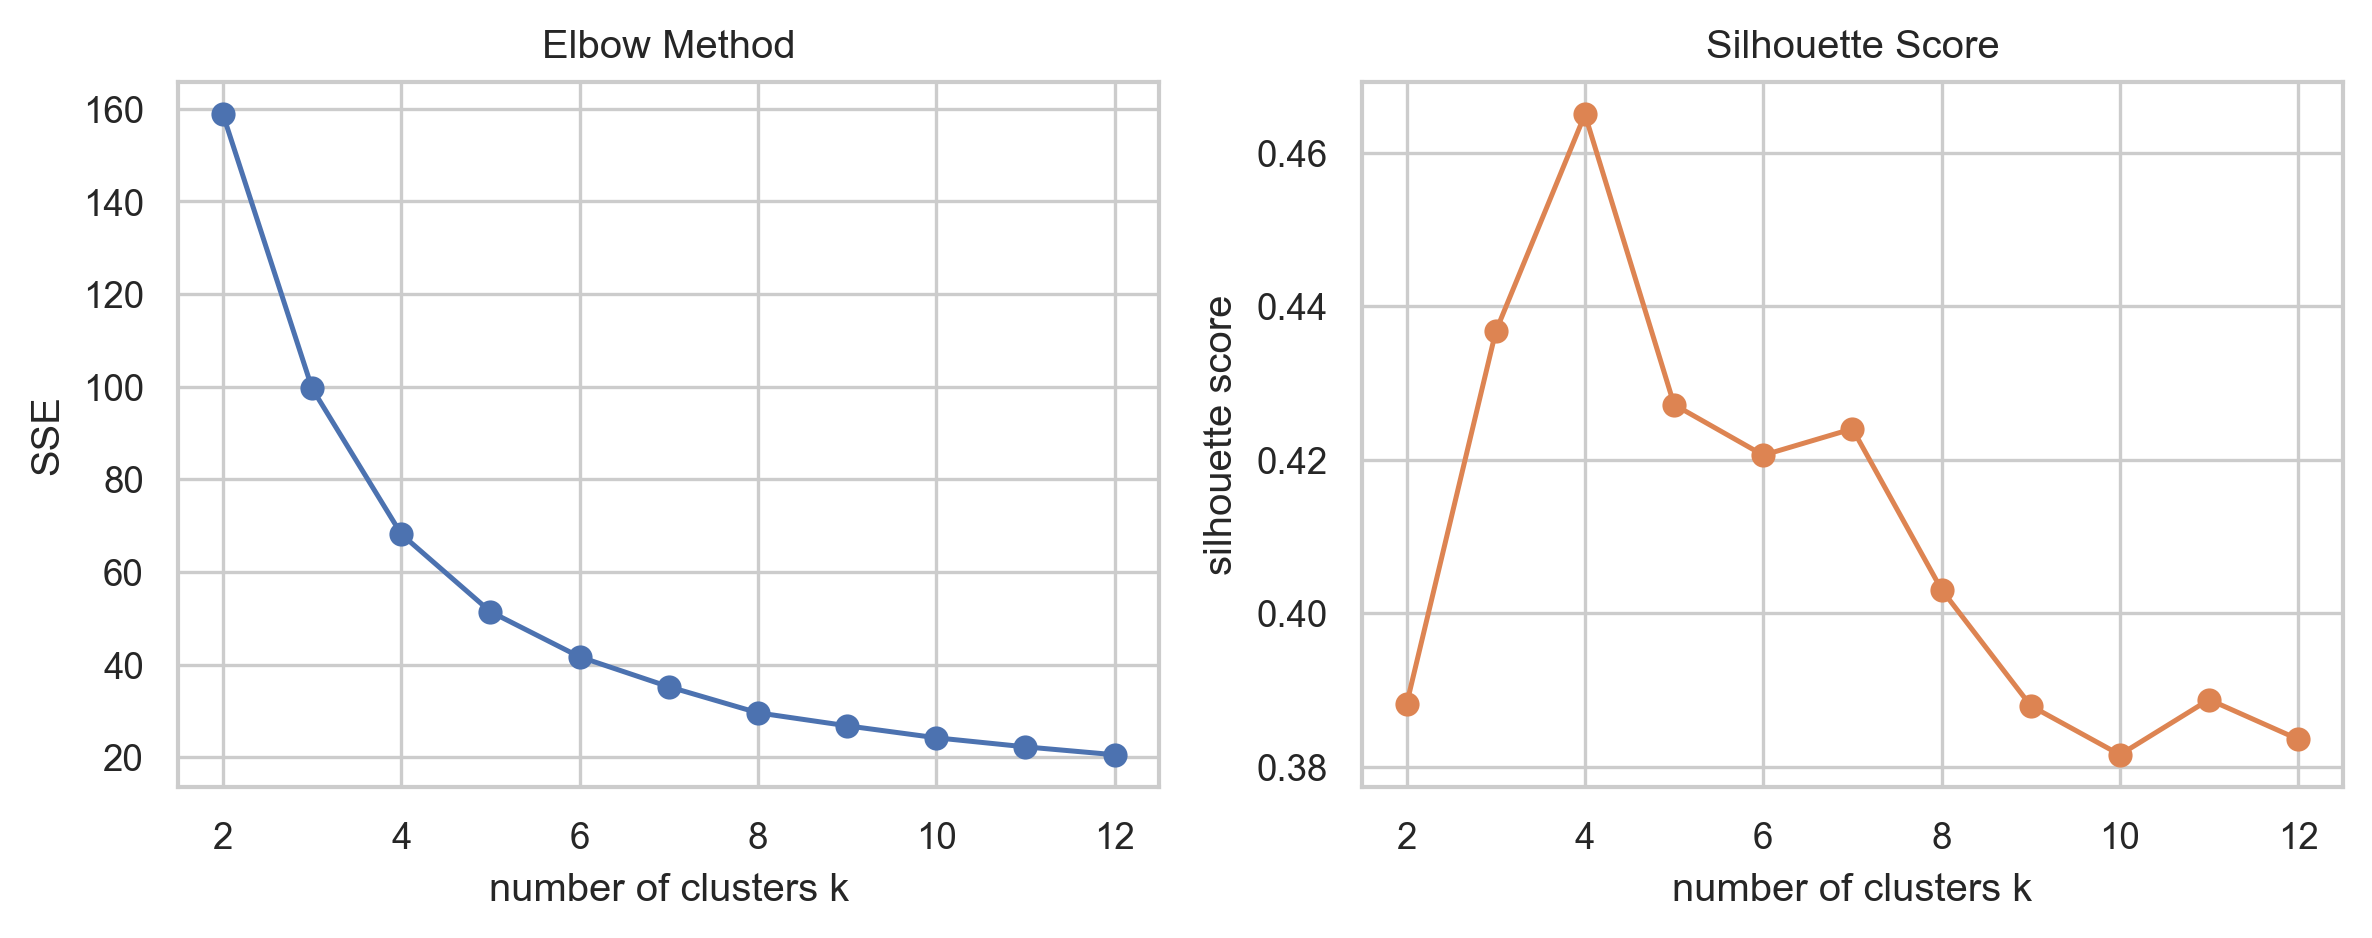
\includegraphics[width=\linewidth]{kmeans_diagnostics.png}
\caption{Elbow (left) and Silhouette (right). $k\!=\!4$ peaks the silhouette.}
\label{fig:diagnostics}
\end{subfigure}\hfill
\begin{subfigure}{0.32\linewidth}\centering
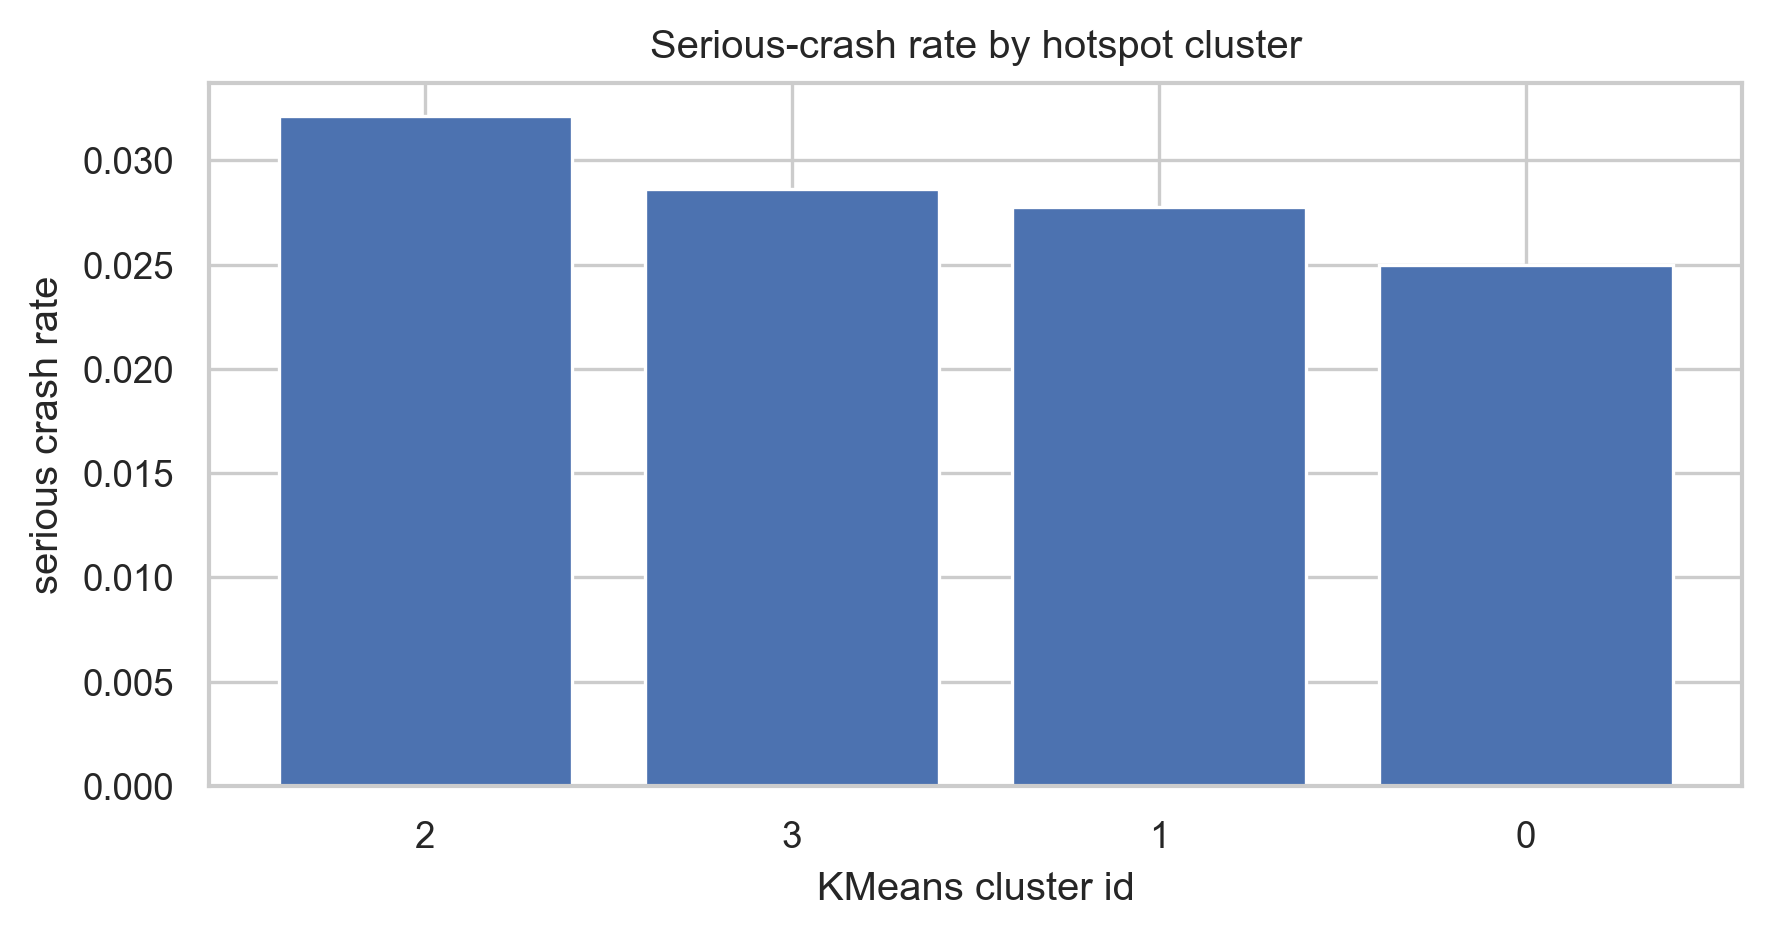
\includegraphics[width=\linewidth]{severity_by_cluster.png}
\caption{Serious rate per cluster (28\% gap).}
\label{fig:cluster_severity}
\end{subfigure}
\caption{KMeans diagnostics and resulting cluster-level serious-crash rates.}
\end{figure}

\begin{figure}[h]
\centering
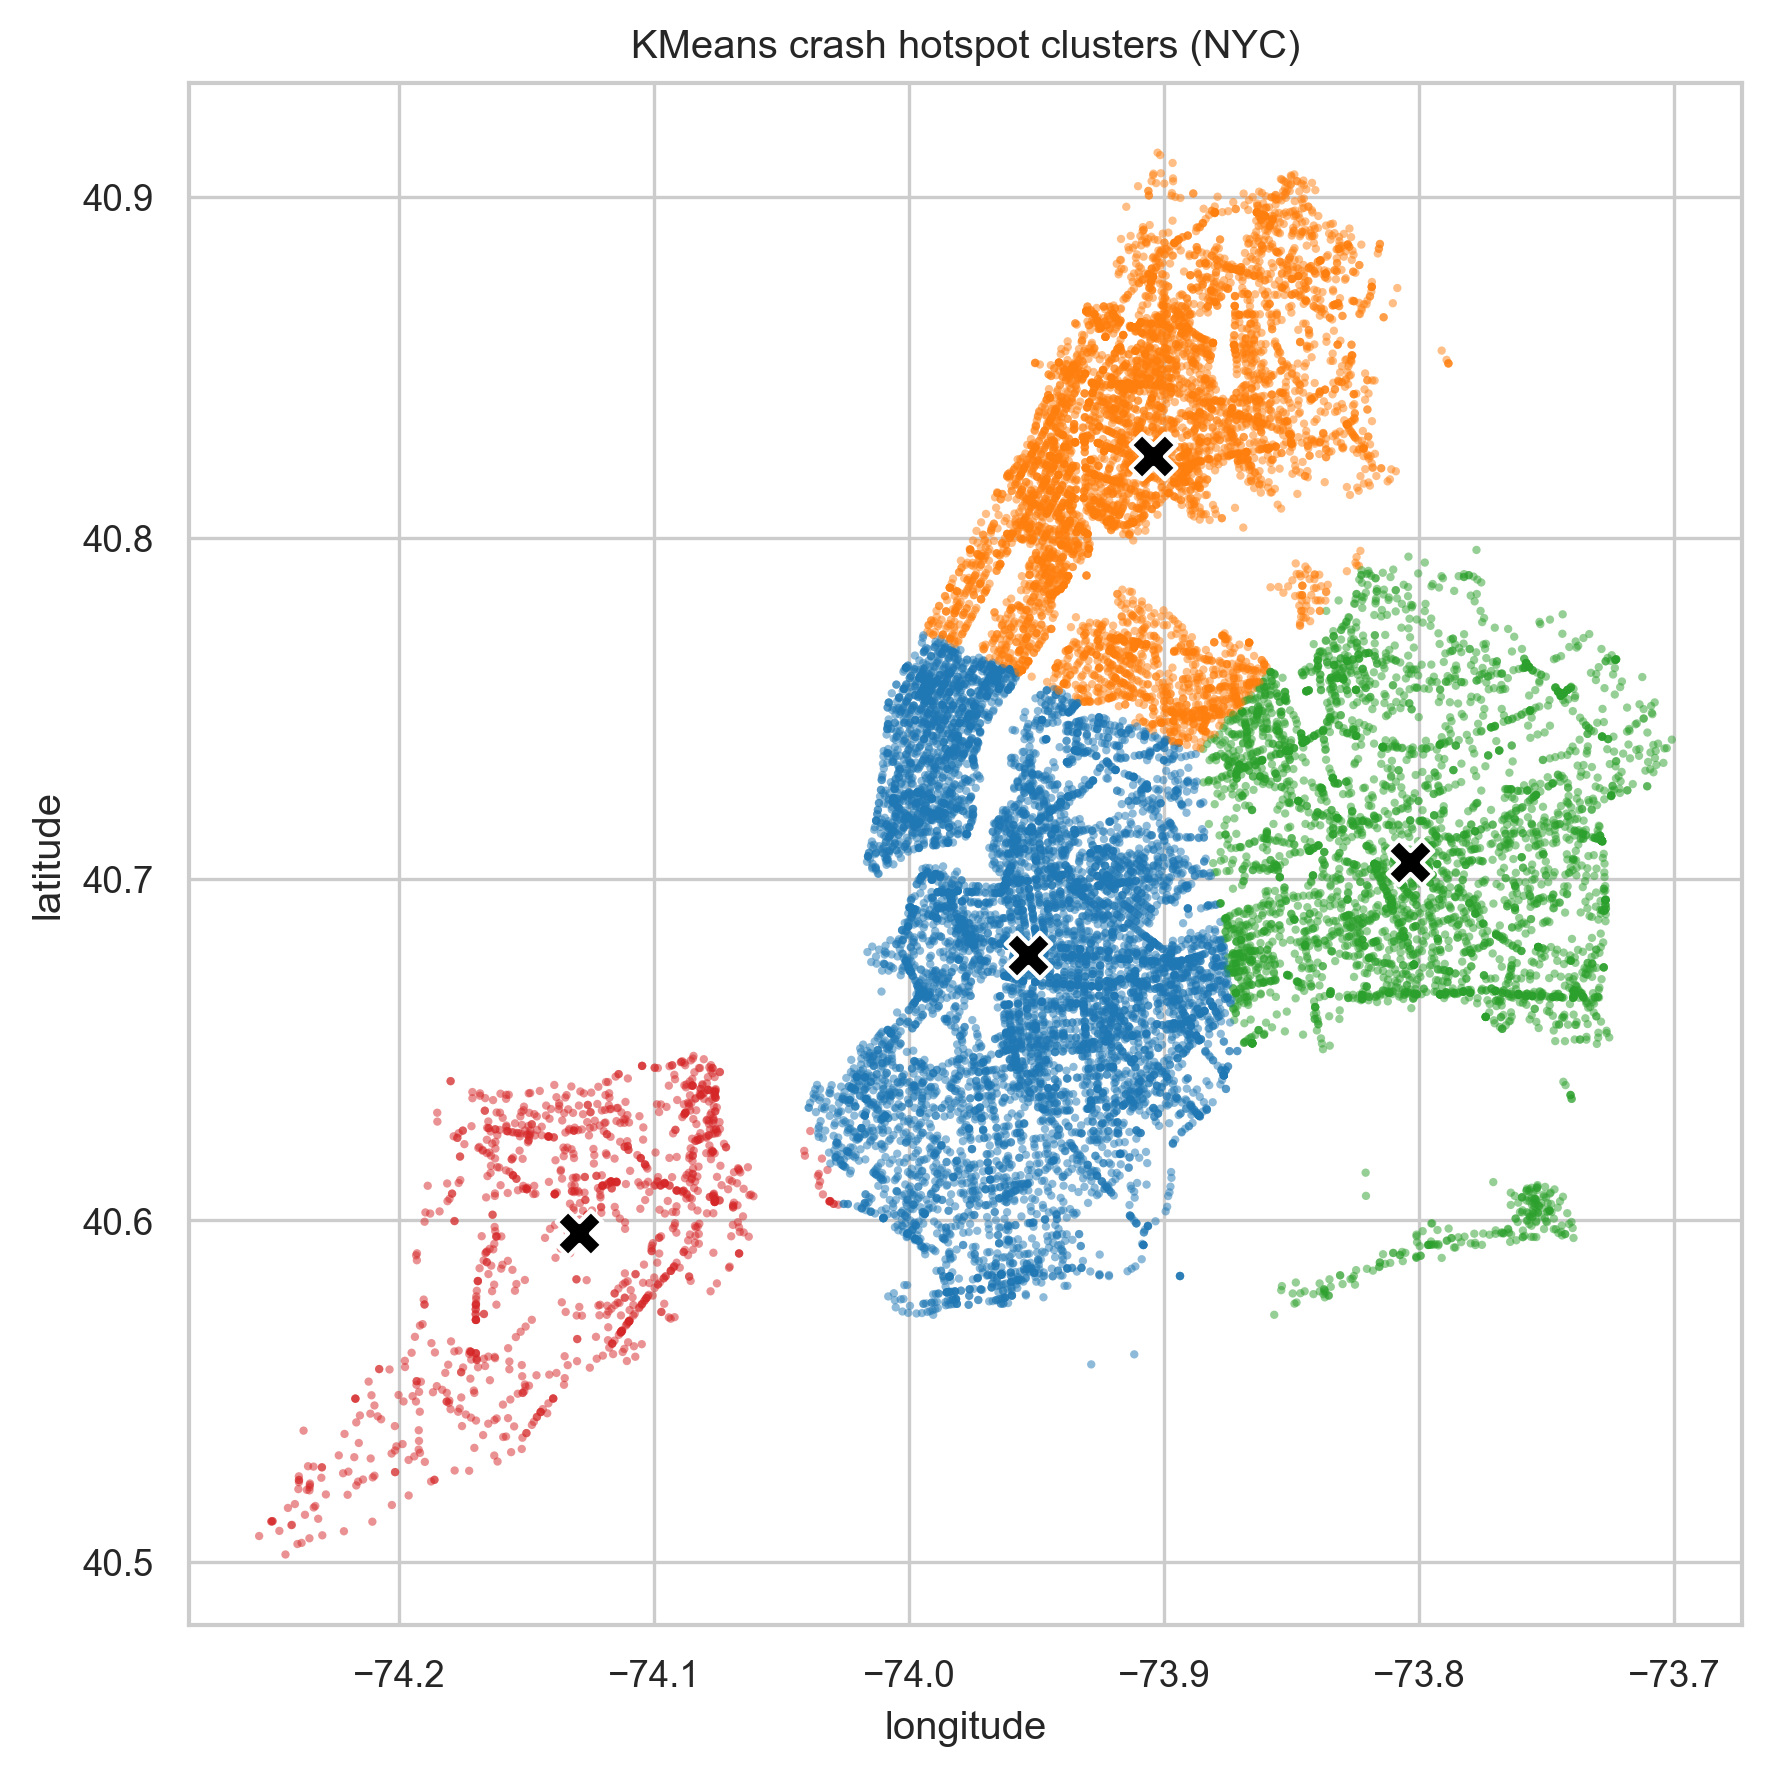
\includegraphics[width=0.42\linewidth]{kmeans_clusters_map.png}
\caption{KMeans cluster assignment with centroids (black X). 20{,}000-crash
random sample of the test fold.}
\label{fig:cluster_map}
\end{figure}

Table~\ref{tab:borough} confirms that borough-level patterns broadly agree with
the cluster-level analysis. Manhattan, despite being the densest crash area,
has the \emph{lowest} serious rate (1.51\%); the Bronx, Brooklyn, and Staten
Island sit between 2.5\% and 2.6\%. Table~\ref{tab:zip} shows the top 10 ZIP
codes by serious-crash count -- concentrated in Brooklyn and Queens (with
one Bronx ZIP, 10469), consistent with the KMeans hotspots in
Figure~\ref{fig:cluster_map}.

\begin{table}[h]
\centering
\caption{Borough-level totals and serious-crash rates (full 2021--2022).}
\label{tab:borough}
\begin{tabular}{lrrr}
\toprule
Borough & Total & Serious & Serious \% \\
\midrule
Bronx          & 24{,}395 & 625   & 2.56 \\
Brooklyn       & 46{,}564 & 1{,}183 & 2.54 \\
Staten Island  & 5{,}111  & 129   & 2.52 \\
Queens         & 36{,}376 & 855   & 2.35 \\
Manhattan      & 22{,}240 & 336   & 1.51 \\
\bottomrule
\end{tabular}
\end{table}

\begin{table}[h]
\centering
\caption{Top 10 ZIP codes by serious-crash count (\(\geq 50\) total crashes).}
\label{tab:zip}
\begin{tabular}{lrrr}
\toprule
ZIP & Total & Serious & Serious \% \\
\midrule
11207 & 3{,}658 & 127 & 3.47 \\
11236 & 2{,}367 &  99 & 4.18 \\
11234 & 1{,}984 &  92 & 4.64 \\
11212 & 2{,}358 &  73 & 3.10 \\
11208 & 2{,}272 &  64 & 2.82 \\
10469 & 1{,}264 &  64 & 5.06 \\
11203 & 2{,}024 &  63 & 3.11 \\
11434 & 1{,}534 &  52 & 3.39 \\
11413 & 1{,}114 &  52 & 4.67 \\
11226 & 1{,}774 &  45 & 2.54 \\
\bottomrule
\end{tabular}
\end{table}

\subsection{Severity Prediction Results}
Table~\ref{tab:summary} summarizes test-set performance for all models on the
\textsc{full} feature set, plus the majority-class baseline. The headline
findings are:

\begin{itemize}
\item \textbf{Accuracy is misleading.} The majority baseline already
achieves 0.970 accuracy because the serious class is only 3\% of the test
set. Random Forest and XGBoost+SMOTE both collapse to near-majority
predictions, recovering accuracy at the cost of zero serious recall.
\item \textbf{Balanced accuracy and recall favor Logistic Regression.} The
class-weighted logistic regression has the best balanced accuracy (0.585) and
the best recall on the serious class (0.623). It does so at the cost of low
precision (0.041), generating many false alarms -- this is exactly the
recall-precision tradeoff a deployed risk-flagging system has to negotiate.
\item \textbf{PR-AUC is essentially flat across capacities.} Logistic
Regression's PR-AUC (0.045) is statistically indistinguishable from
XGBoost's (0.042) on this imbalanced task; Random Forest edges out XGBoost on
ROC-AUC (0.593 vs.\ 0.588) but neither offers a meaningful gain over the
linear baseline.
\item \textbf{Threshold tuning trades recall for precision.} Selecting
$\tau\!=\!0.69$ on the validation slice (rather than the default 0.5) lowers
XGBoost's F1 on the serious class from 0.080 to 0.047 but raises precision
from 0.048 to 0.056.
\item \textbf{SMOTE hurts.} Synthetic minority oversampling collapses the
model to majority predictions, consistent with prior reports that SMOTE on
high-cardinality engineered features can blur decision boundaries
\cite{he2009imbalanced}.
\end{itemize}

\begin{table}[h]
\centering
\caption{Severity-prediction test-set metrics (\textsc{full} feature set unless
otherwise noted). PR-AUC and balanced accuracy are the headline metrics under
imbalance.}
\label{tab:summary}
\setlength{\tabcolsep}{4pt}
\begin{tabular}{lrrrrrrr}
\toprule
Model & Acc. & Bal.\,Acc. & P (1) & R (1) & F1 (1) & PR-AUC & ROC-AUC \\
\midrule
Majority baseline           & 0.970 & 0.500 & 0.000 & 0.000 & 0.000 & --     & --     \\
Logistic Regression         & 0.550 & \textbf{0.585} & 0.041 & \textbf{0.623} & 0.077 & \textbf{0.045} & \textbf{0.615} \\
Random Forest               & 0.969 & 0.501 & 0.115 & 0.003 & 0.005 & 0.044 & 0.593 \\
XGBoost                     & 0.837 & 0.544 & 0.048 & 0.231 & 0.080 & 0.042 & 0.588 \\
XGBoost + SMOTE             & 0.969 & 0.500 & 0.091 & 0.001 & 0.002 & 0.040 & 0.583 \\
XGBoost + Threshold ($\tau\!=\!0.69$) & 0.950 & 0.510 & 0.056 & 0.041 & 0.047 & 0.042 & 0.588 \\
\bottomrule
\end{tabular}
\end{table}

Figure~\ref{fig:pr_roc} shows the precision-recall and ROC curves for the
three XGBoost variants. The PR curves remain flat and close to the random
baseline, confirming the difficulty of the task; the ROC curves stay above the
diagonal but only modestly. Figure~\ref{fig:confusion} shows the corresponding
confusion matrices: SMOTE collapses to majority predictions, default XGBoost
flags many crashes as serious (high recall, many false positives), and the
threshold-tuned XGBoost lands between the two with a much smaller false-positive
count.

\begin{figure}[h]
\begin{subfigure}{0.62\linewidth}\centering
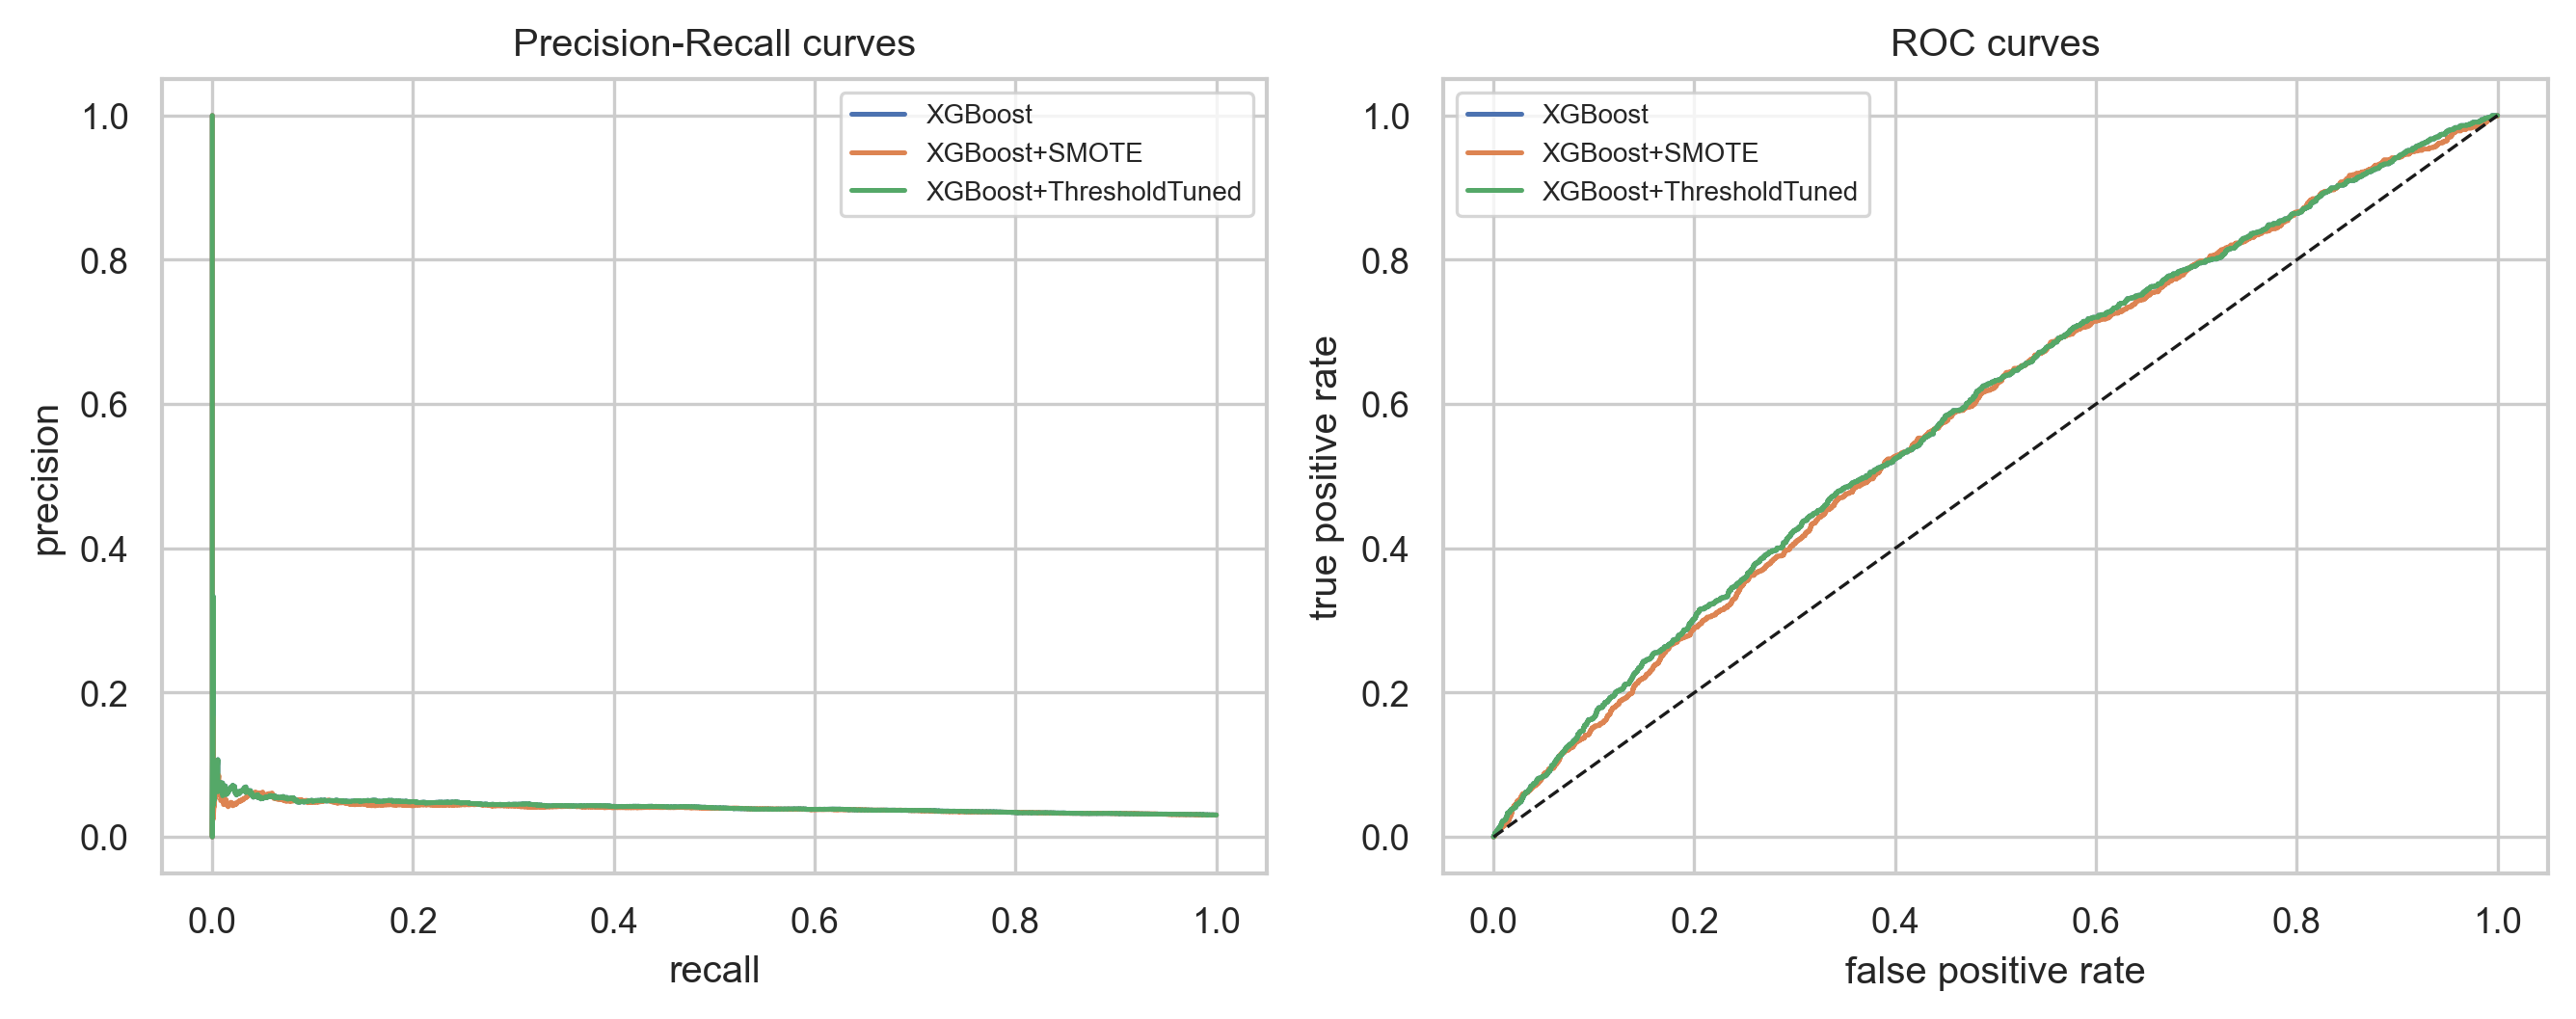
\includegraphics[width=\linewidth]{pr_roc_curves.png}
\caption{PR (left) and ROC (right) curves for the three XGBoost variants.}
\label{fig:pr_roc}
\end{subfigure}\hfill
\begin{subfigure}{0.36\linewidth}\centering
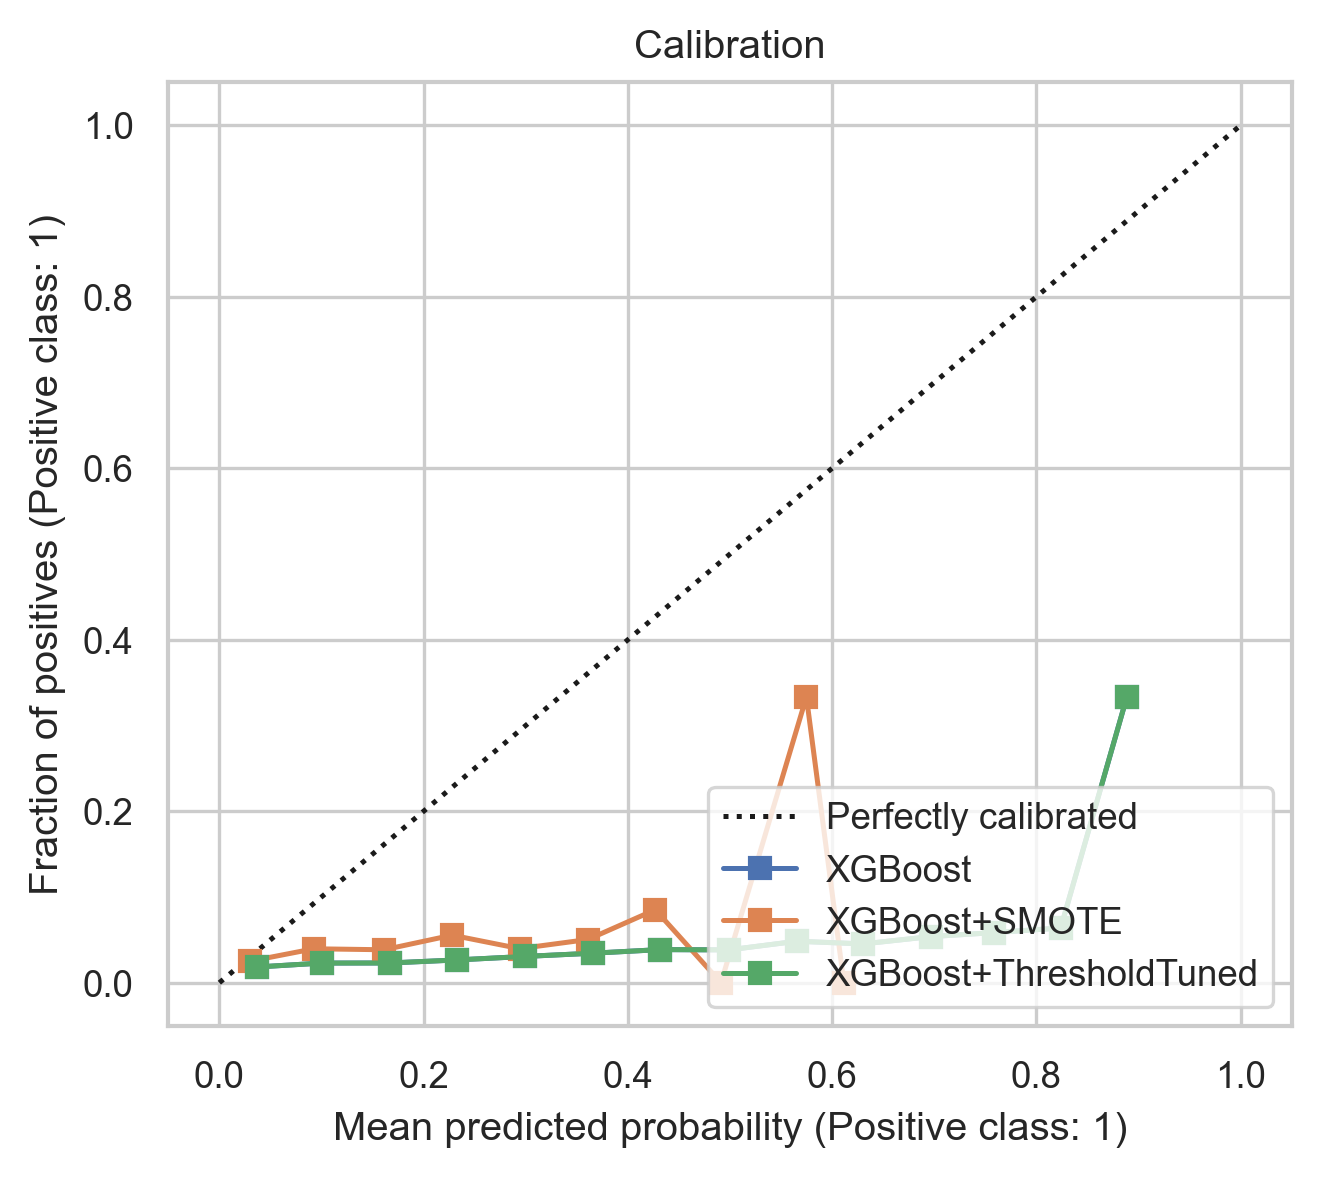
\includegraphics[width=\linewidth]{calibration.png}
\caption{Calibration curves.}
\label{fig:calibration}
\end{subfigure}
\caption{Test-set diagnostics for the XGBoost variants.}
\end{figure}

\begin{figure}[h]
\centering
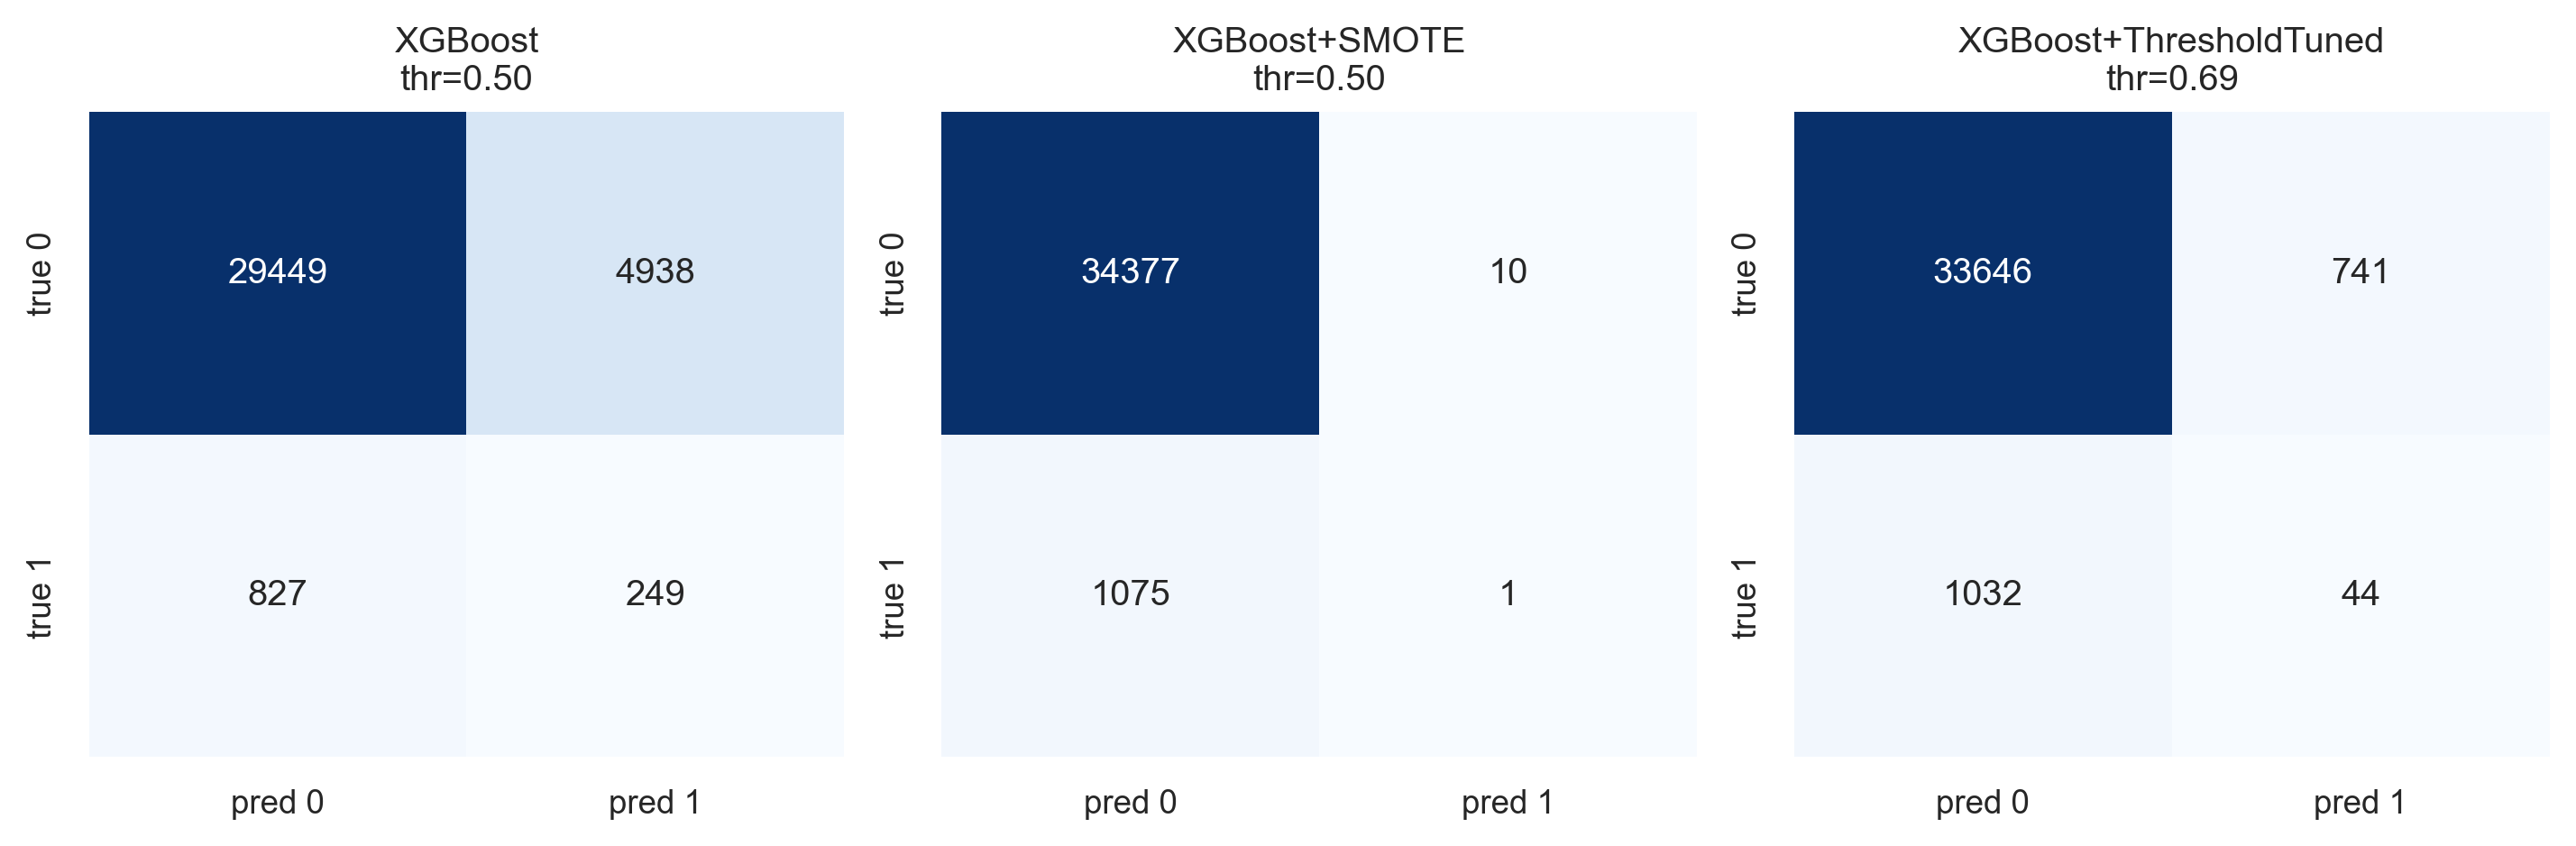
\includegraphics[width=0.85\linewidth]{confusion_matrices.png}
\caption{Confusion matrices for the three XGBoost variants. Among imbalance
treatments, threshold tuning is the only one that avoids the SMOTE collapse to
majority predictions while keeping the false-positive count manageable.}
\label{fig:confusion}
\end{figure}

\subsection{Feature-Group Ablation}
Table~\ref{tab:ablation} reports XGBoost performance across the four feature
sets. Adding weather features yields a small accuracy gain
(0.790 $\to$ 0.839) and a slight PR-AUC bump
(0.043 $\to$ 0.044); adding the radial spatial feature yields no additional
benefit; adding cluster identity yields no benefit either, and in fact slightly
hurts PR-AUC (0.044 $\to$ 0.042).

This is an interpretable negative result: gradient boosting can already extract
spatial structure from the raw lat/lon coordinates, so a coarse 4-bin cluster
identity is redundant. The cluster identity may still be valuable for
downstream interpretability and for linear models like Logistic Regression
(which gain a small bump in balanced accuracy when cluster id is added; see
Tab.~\ref{tab:summary}).

\begin{table}[h]
\centering
\caption{XGBoost feature-group ablation. Weather contributes a small accuracy
gain; spatial radial and cluster identity are redundant for tree-based models.}
\label{tab:ablation}
\begin{tabular}{lrrrrr}
\toprule
Feature set & Acc. & Bal.\,Acc. & PR-AUC & ROC-AUC & Recall (1) \\
\midrule
time-only                          & 0.790 & 0.557 & 0.043 & 0.598 & 0.309 \\
\,+weather                         & 0.839 & 0.555 & 0.044 & 0.588 & 0.252 \\
\,+spatial                         & 0.830 & 0.554 & 0.044 & 0.592 & 0.261 \\
\,+cluster (full)                  & 0.837 & 0.544 & 0.042 & 0.588 & 0.231 \\
\bottomrule
\end{tabular}
\end{table}

\subsection{PCA and SHAP Interpretability}
Figure~\ref{fig:pca_shap} (left) projects the engineered numeric feature set
onto its first two principal components: the serious class spreads across the
projection rather than forming a separable cluster, which matches the modest
PR-AUC numbers in Table~\ref{tab:summary}. Figure~\ref{fig:pca_shap} (right)
reports the SHAP feature-importance bar plot for the \textsc{full}-feature
XGBoost. Time and spatial features dominate (\texttt{hour}, $\sin/\cos$
encodings, latitude, longitude, distance to midtown); weather features
contribute meaningful but lower-ranked attributions
(\texttt{precipitation}, \texttt{cloud\_pct}, \texttt{temp\_max}); cluster-id
one-hot variables rank near the bottom, consistent with
Table~\ref{tab:ablation}.

\begin{figure}[!htb]
\begin{subfigure}{0.36\linewidth}\centering
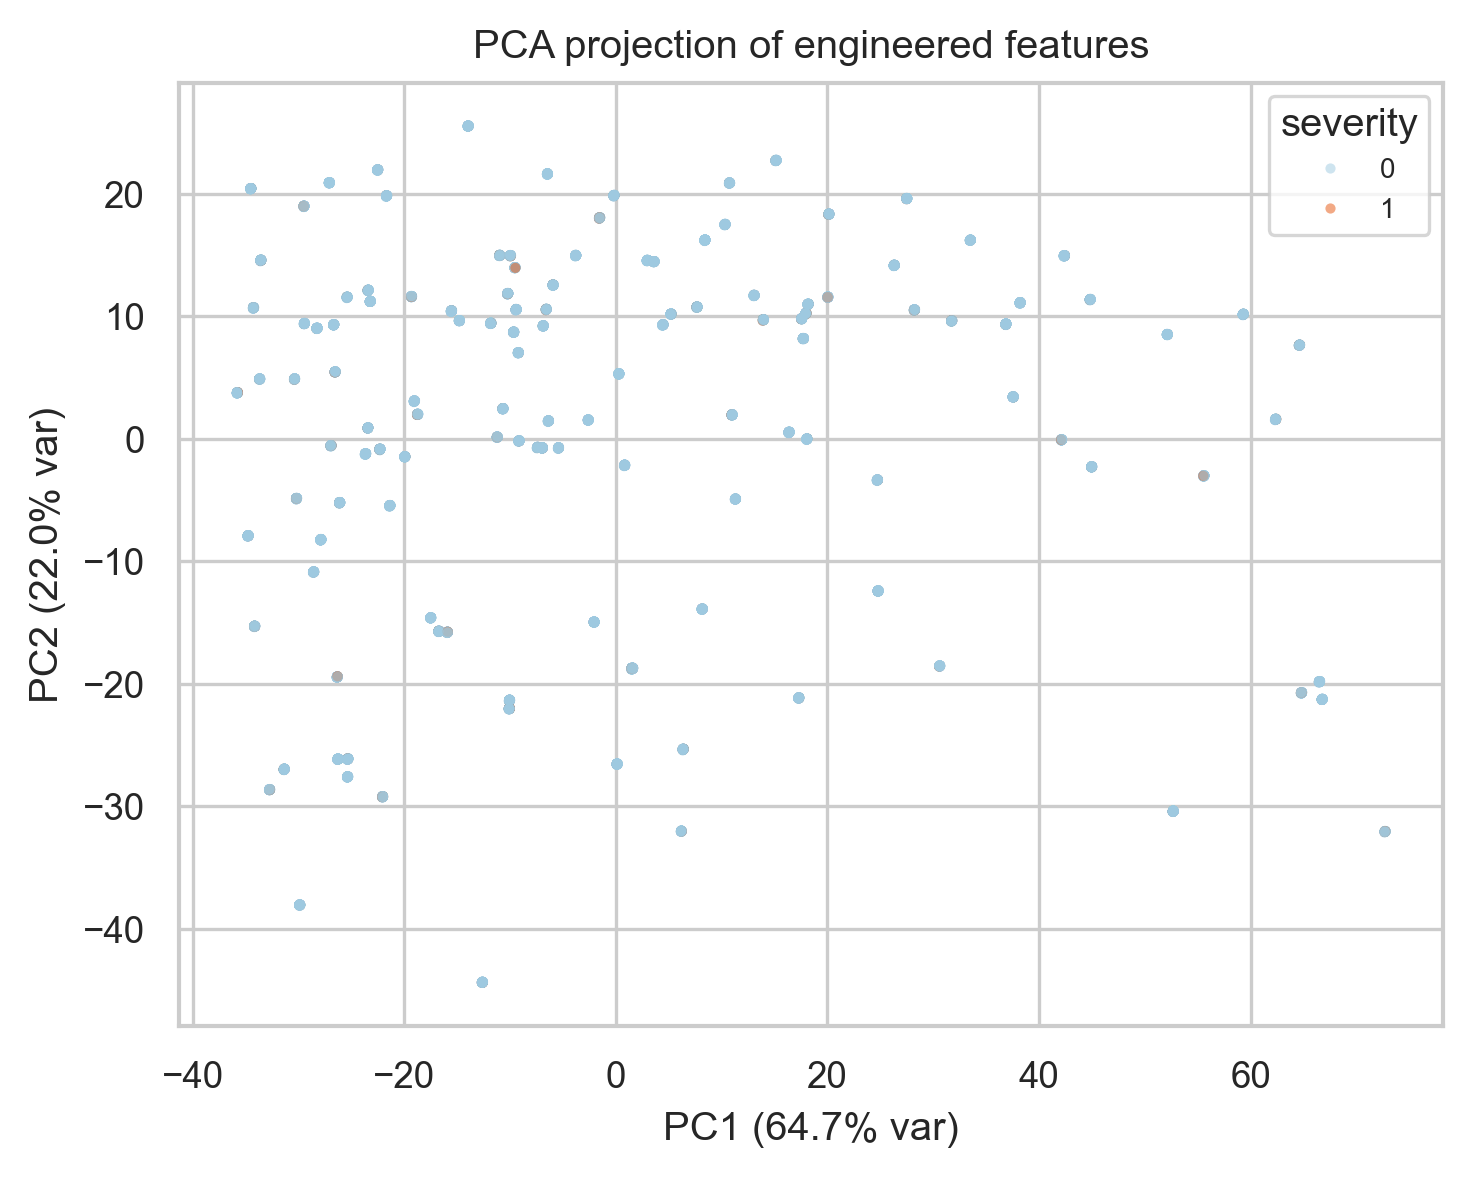
\includegraphics[width=\linewidth]{pca_projection.png}
\caption{PCA of engineered features (test set) by ground-truth severity.}
\end{subfigure}\hfill
\begin{subfigure}{0.50\linewidth}\centering
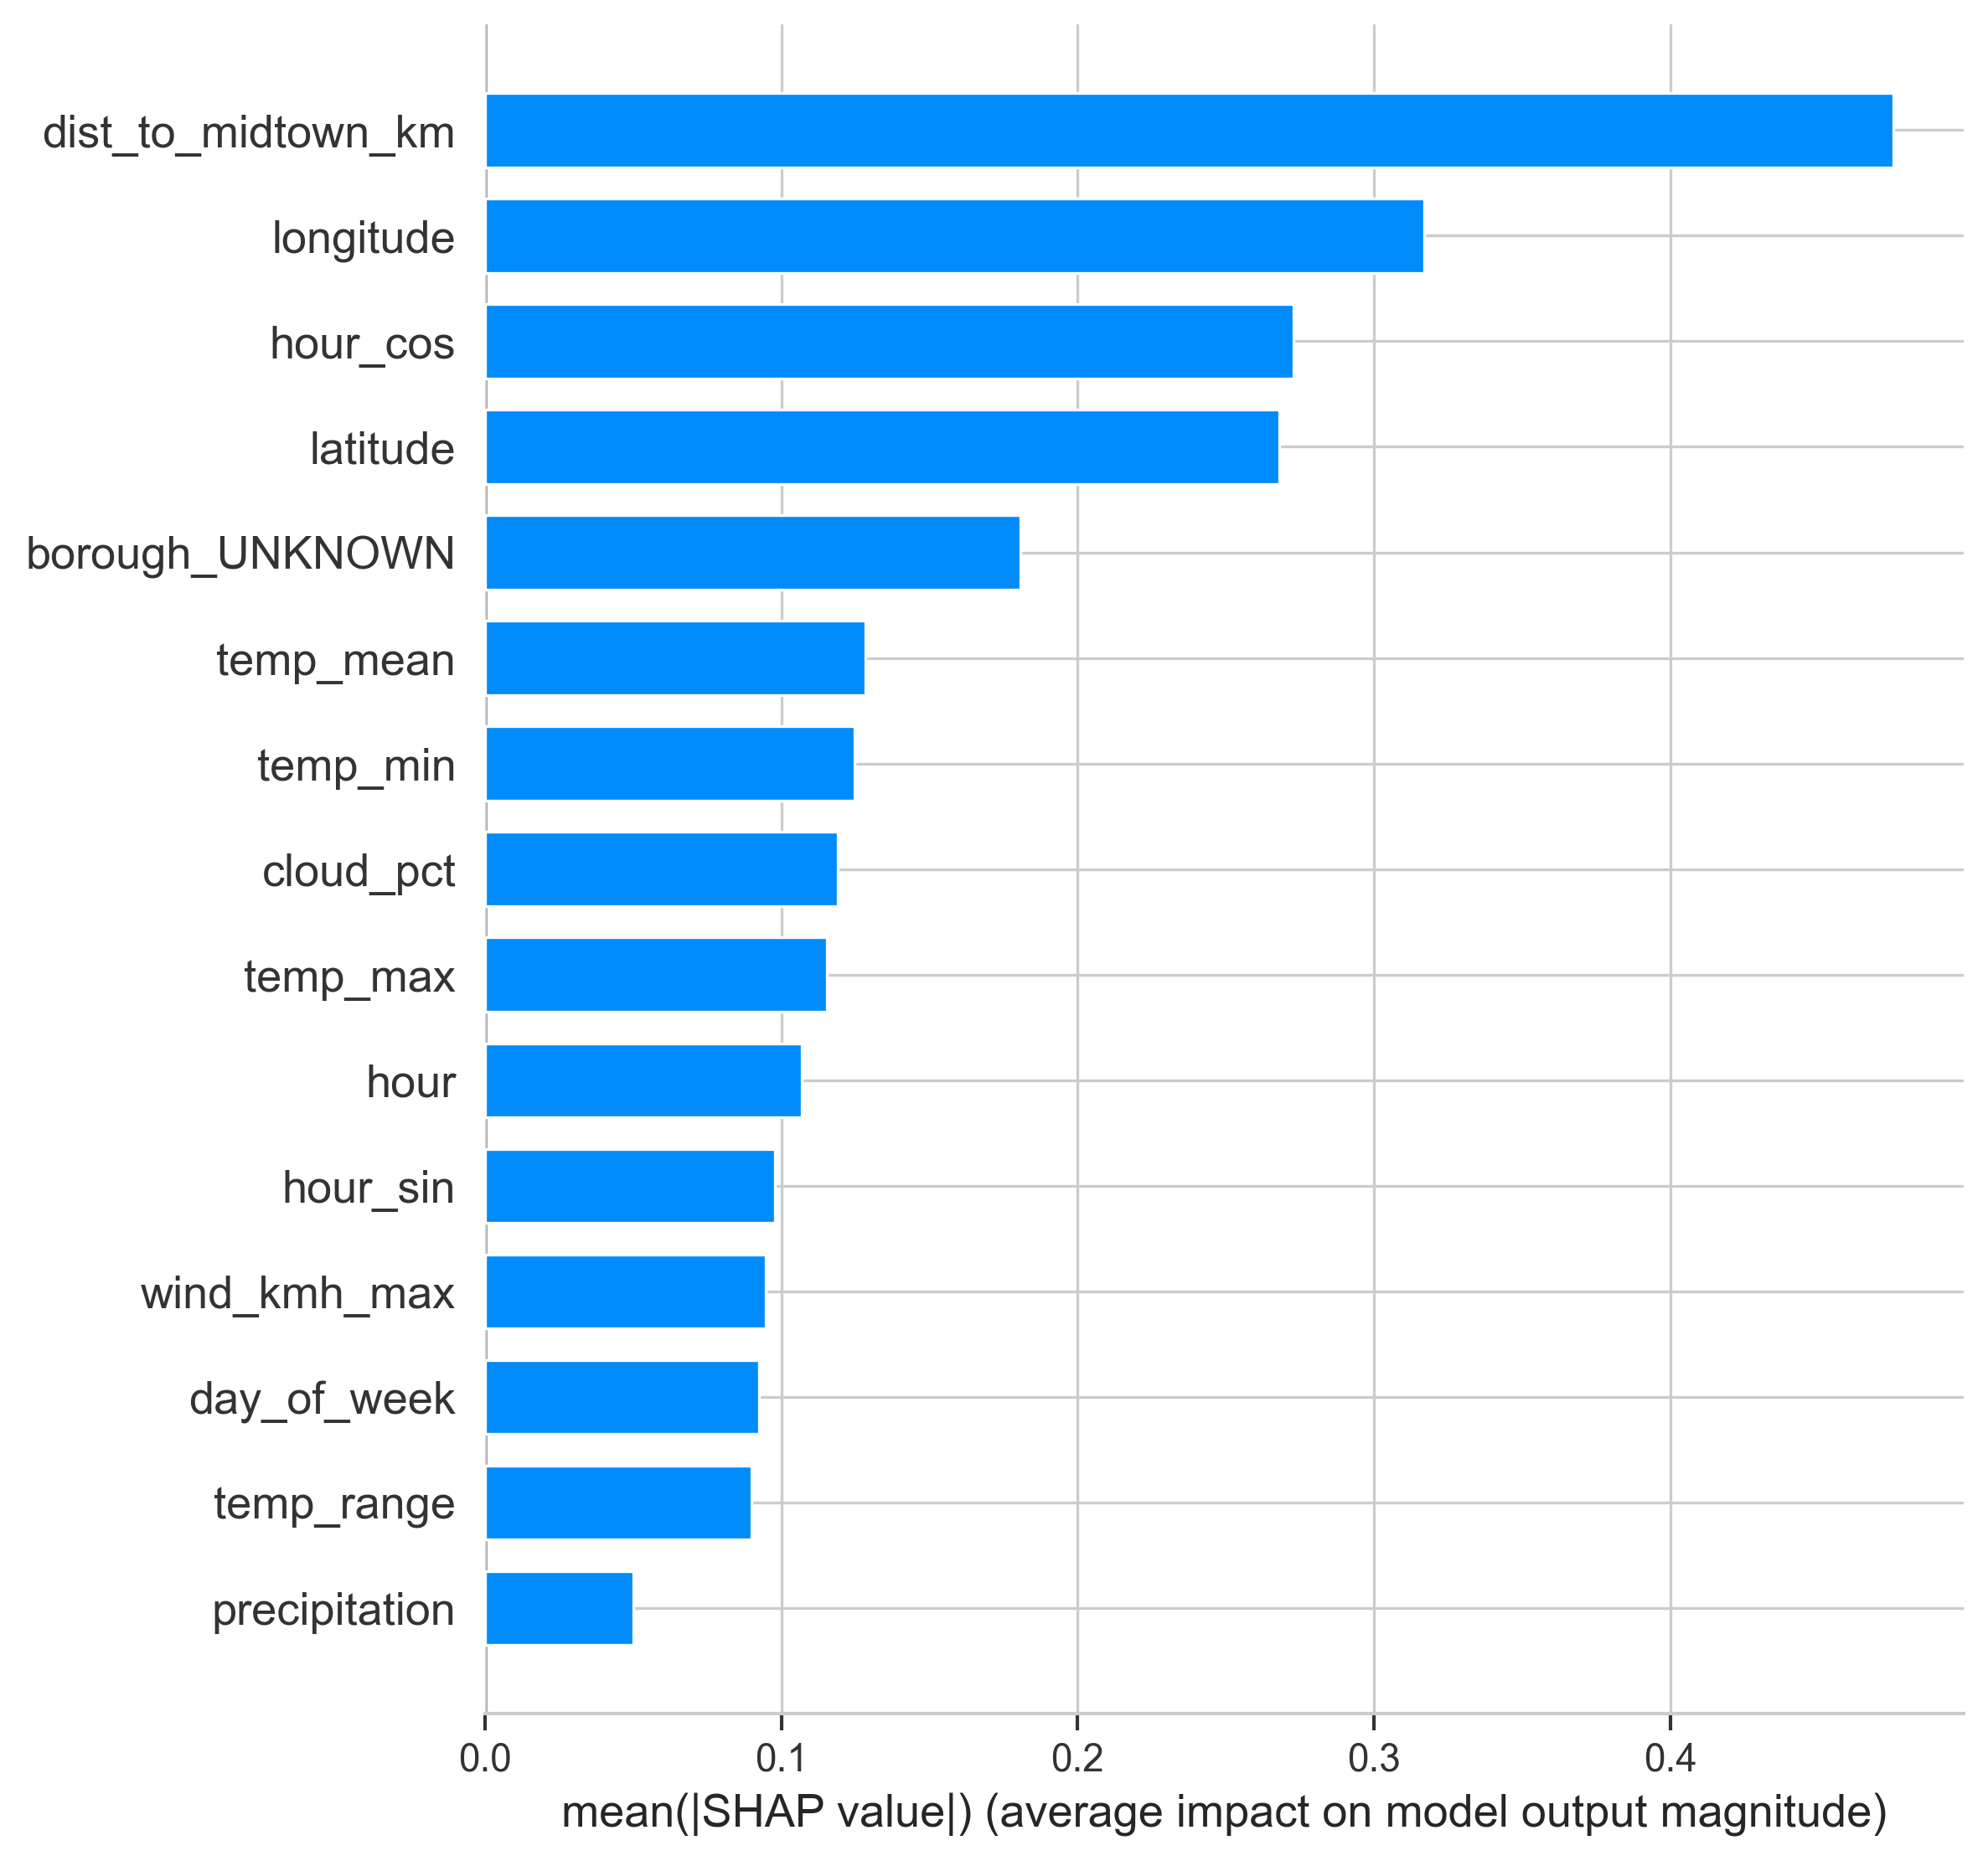
\includegraphics[width=\linewidth]{shap_summary.png}
\caption{SHAP feature-importance bar plot, \textsc{full}-feature XGBoost.}
\end{subfigure}
\caption{Interpretability diagnostics for the trained XGBoost classifier.}
\label{fig:pca_shap}
\end{figure}

\FloatBarrier
\section{Discussion and Conclusion}
\label{sec:discussion}

Three findings stand out from this hybrid pipeline.
\textbf{Hotspot discovery is informative}: the KMeans clusters span an
approximately 28\% relative gap in \mbox{serious-crash} rate and are
corroborated by the borough/ZIP analysis. \textbf{Recall is dominated by the
imbalance treatment, not model capacity}: no model in the ladder reaches
PR-AUC above 0.045, and a class-weighted Logistic Regression edges out the
non-linear ensembles on balanced accuracy and PR-AUC -- consistent with the
imbalanced-learning literature~\cite{he2009imbalanced} and attributable to
the absence of causal features (vehicle speed/type, driver profile, road
geometry). \textbf{Cluster identity is largely redundant for gradient
boosting}, which already extracts spatial structure from raw
$(\mathrm{lat},\mathrm{lon})$; the cluster id remains useful for linear
models and for human-readable communication.

\paragraph{Limitations and future work.}
Dominant limitations are class imbalance with missing causal features, daily
weather granularity, coordinate bias, and a two-year temporal scope.
Promising next steps include hourly weather joins, NYC LION road features
and DOT traffic counts~\cite{theofilatos2014review}, a learnable
spatio-temporal grid, and a cost-sensitive evaluation metric for Vision Zero
deployment.

\section*{Contributions}
Pranav Arra (psa39): literature review and ablation design. Logan Sharrott
(ls1428): unsupervised clustering and SHAP/PCA interpretability. Vishal
Nagamalla (vn218): ETL pipeline, training ladder, and reproducibility. All
three authors co-wrote the report.

\bibliographystyle{plainnat}
\bibliography{refs}

\end{document}
